\documentclass{acmsiggraph}                     % final
%\documentclass[annualconference]{acmsiggraph}  % final (annual conference)
%\documentclass[review]{acmsiggraph}            % review
%\documentclass[widereview]{acmsiggraph}        % wide-spaced review
%\documentclass[preprint]{acmsiggraph}          % preprint

\usepackage[ngerman]{babel}
\usepackage[utf8]{inputenc}
\usepackage[T1]{fontenc}
\usepackage{amssymb}

\usepackage[scaled=.92]{helvet}
\usepackage{times}

\usepackage{microtype}

\usepackage{graphicx}

\usepackage{siunitx}
\usepackage{parskip}

\usepackage[labelfont=bf,textfont=it]{caption}

\usepackage{amsmath}
\usepackage{subfigure}

\usepackage[colorlinks=true,linkcolor=black,citecolor=black,urlcolor=black,pdfauthor={Benjamin Glatzel und Dominik Wilhelm}]{hyperref}

\usepackage{listings}
\usepackage{color}
\definecolor{lightgray}{rgb}{.92,.92,.92}
\definecolor{keyword}{rgb}{.0,.48,.65}

\lstset{
	basicstyle=\footnotesize\ttfamily,
	captionpos=b,
	numbers=left,
	numberstyle=\tiny,
	numbersep=5pt,
	tabsize=2,
	extendedchars=true,
	breaklines=true,
	% keywordstyle=\color{keyword},
	showstringspaces=false,    
	showspaces=false,
	showtabs=false,
	backgroundcolor=\color{lightgray}
}

\lstdefinelanguage{pseudo}{
    keywords={set, for, end, return, to, of, at, do, and, vertex, program, with, parameters, fragment,in,pixel,each,saturate,absolute},
	comment=[l]{//}
}

\graphicspath{{Bilder/}}

\title{Nutzung von Echtzeit-Tiefenschärfe-Effekten zur Beeinflussung von wahrgenommenen Größen- sowie Abstandsverhältnissen}

\author{Benjamin Glatzel\thanks{E-Mail: benjamin.glatzel@me.com}\\ Hochschule Darmstadt
\and Dominik Wilhelm\thanks{E-Mail: dominik\_wilhelm@arcor.de}\\ Hochschule Darmstadt}

\keywords{Tiefenschärfe, Echtzeit, Shader, Tilt-Shift-Effekt}

\begin{document}

\teaser{
	\subfigure[]{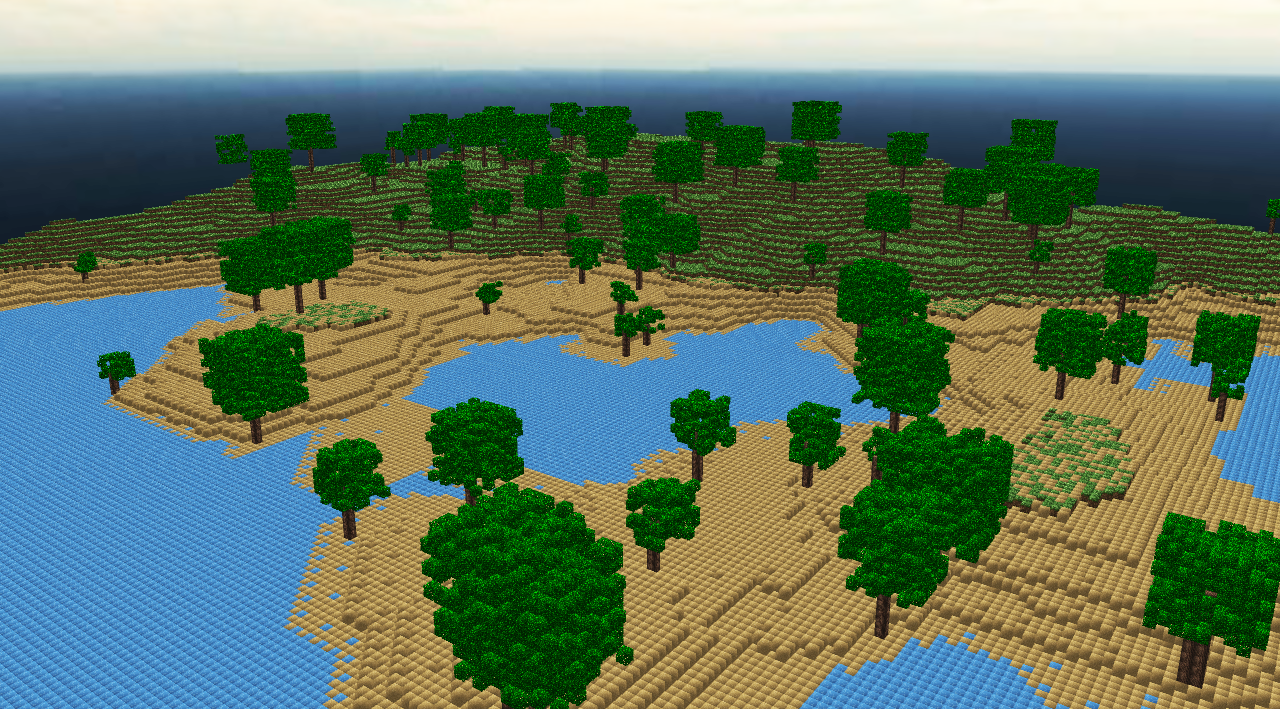
\includegraphics[width=3.3in]{Blockcraft-1-Original}}
	\qquad
 	\subfigure[]{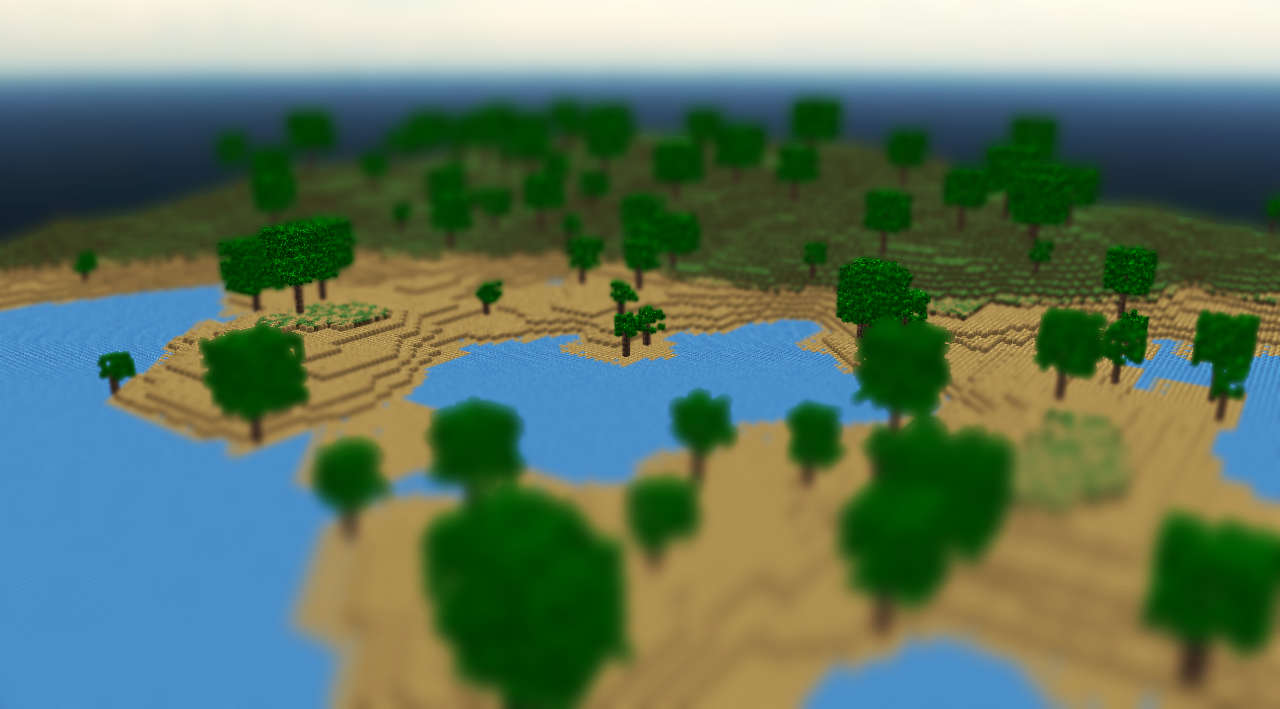
\includegraphics[width=3.3in]{Blockcraft-1-Blur}}
  	\caption{Die linke Abbildung zeigt eine Aufnahme der Beispielszene, bei der die Distanz zur Schärfeebene auf $\SI{75.0}{\meter}$ eingestellt und sowohl die Brennweite als auch die Größe der Linse an die Eigenschaften des menschlichen Auges angepasst wurden. Innerhalb der rechten Abbildung wurde die Größe der Linse so angepasst, dass ein Abstand von $\SI{6.0}{\centi\meter}$ zur Schärfeebene simuliert wird. Nach Anwendung des in diesem Paper vorgestellten Algorithmus, wirken die Bäume und das Terrain innerhalb der Szene merklich miniaturisiert. }
	\label{teaser}
}

\maketitle

\def\abstractname{Abstract}
\begin{abstract}

Innerhalb des vorliegenden Papers wird ein Algorithmus vorgestellt, der die Manipulation von wahrgenommenen Größen- und Abstandsverhältnissen in Echtzeit ermöglicht. Hierzu wird ein Modell zur Berechnung von Tiefenschärfe eingeführt, das mithilfe von Shadern und einem Grafikchip effizient zur Berechnung verwendet werden kann. Die Anwendung des Algorithmus für die Erzeugung des sogenannten Tilt-Shift-Effektes unter Berücksichtigung der menschlichen Wahrnehmung lieferte gute Ergebnisse und wurde anhand einer speziellen, fraktal generierten Beispielszene erprobt und validiert. Auch der Vergleich mit Offline-Verfahren war zufriedenstellend und zeigte lediglich die erwarteten, durch die Unterschiedlichkeiten der Berechnung bedingten, Differenzen.

% \begin{eqnarray}
% x & \ll & y_{1} + \cdots + y_{n} \\
%   & \leq & z
% \end{eqnarray}

% Citations can be done this way~\cite{Jobs95} or this more concise 
% way~\shortcite{Jobs95}, depending upon the application.

\end{abstract}

\keywordlist

\section{Einleitung}

\copyrightspace

Unschärfe in Fotografien und Grafiken kann wahrgenommene Größen- und Abstandsverhältnisse merklich beeinflussen~\cite{Held:2010cr}. Dieses Phänomen kann einerseits dazu verwendet werden, Szenen viel größer wirken zu lassen, als sie tatsächlich sind, oder aber für die Miniaturisierung von Motiven eingesetzt werden. Der erste Fall wird häufig für Spezialeffekte mithilfe von sehr kleinen Kameraobjektiven, die die Variation und die Intensität von Unschärfe merklich reduzieren, eingesetzt~\cite{Held:2010cr}. Die Miniaturisierung kann mit einer fotografischen Manipulation, dem sogenannten Tilt-Shift-Effekt, erzeugt werden.

Für die Realisierung des Tilt-Shift-Effektes existieren drei bewährte Umsetzungsmöglichkeiten: die Verwendung von Tilt-Shift-Objektiven, die Anwendung eines vertikalen Unschärfefilters durch Postprocessing und die realitätsnahe, physikalische Berechnung von Tiefenschärfe. Während die ersten beiden Möglichkeiten bei Fotografien leicht angewendet werden können, sind für die realitätsnahe Berechnung Tiefeninformationen eine Grundvoraussetzung. Da bei der Entwicklung von Echtzeit-3D-Applikationen Tiefeninformationen ein grundlegender Bestandteil sind und die Ausrichtung eines vertikalen Unschärfefilters geschickt gewählt werden muss, eignet sich in diesem Szenario eine realitätsnahe Berechnung.

Abbildung \ref{teaser} (a) und Abbildung \ref{teaser} (b) zeigen die Ergebnisse nach einer Echtzeit-Tiefenschärfe-Berechnung angewandt auf eine fraktal generierte Beispielszene. Die Parameter wurden für die Generierung der Abbildungen so gewählt, dass, unter Berücksichtigung der Eigenschaften des menschlichen Auges, eine fokussierte Distanz von $\SI{75.0}{\meter}$ auf  $\SI{6.0}{\centi\meter}$

Wie zu erkennen ist, eignen sich Echtzeitverfahren für die Erzeugung des Tilt-Shift-Effektes. Innerhalb des vorliegenden Papers wird ein einfacher Algorithmus beschrieben, der die Berechnung von Tiefenschärfe unter Berücksichtigung der menschlichen Wahrnehmung in Echtzeit ermöglicht. Durch dessen Anwendung können Größenverhältnisse betrachteter Szenen durch Defokussierung und Fokussierung manipuliert und an gewünschte Größenverhältnisse angepasst werden. Abschließend werden die Ergebnisse validiert und mit einer offline Reproduktion verglichen.

\section{Hintergrund}

Die Berechnung von Tiefenschärfe ist in vielerlei Hinsicht bedeutsam. Unschärfe kann dazu eingesetzt werden, den Blick des Betrachters zu steuern und auf bestimmte Bildregionen auszurichten~\cite{Held:2010cr}. Dies kann durch die Scharfzeichnung des zu betrachtenden bzw. zu fokussierenden Objektes und die Weichzeichnung der verbleibenden Bildelemente erreicht werden. Tiefenschärfe eignet sich zudem, wie bereits erwähnt wurde, zur Manipulation von wahrgenommenen Größen- und Abstandsverhältnissen. Einerseits können durch die Nutzung von sehr kleinen Kameraobjektiven Miniaturen so aufgenommen werden, dass diese im Vergleich zum Original deutlich größer wirken. Dieser Effekt wird primär beim Filmdreh verwendet~\cite{Held:2010cr}.

Andererseits hat sich der Tilt-Shift-Effekt zur Umkehrung des Effekts etabliert. Die ursprüngliche Namensgebung stammt von sogenannten Tilt-Shift-Objektiven, die die Ausrichtung der Linse relativ zur Bildebene ermöglichen. Beim Einsatz dieser können unter Berücksichtigung des Scheimpflugprinzips Ebenen in den Fokus gerückt werden, die anderenfalls außerhalb des Fokusbereiches liegen würden~\cite{Held:2010cr}. Umgekehrt können Bereiche aus der Fokusebene bewegt werden, die unter Verwendung eines handelsüblichen Kameraobjektives fokussiert wären.

\begin{figure}[htbp]
\centering
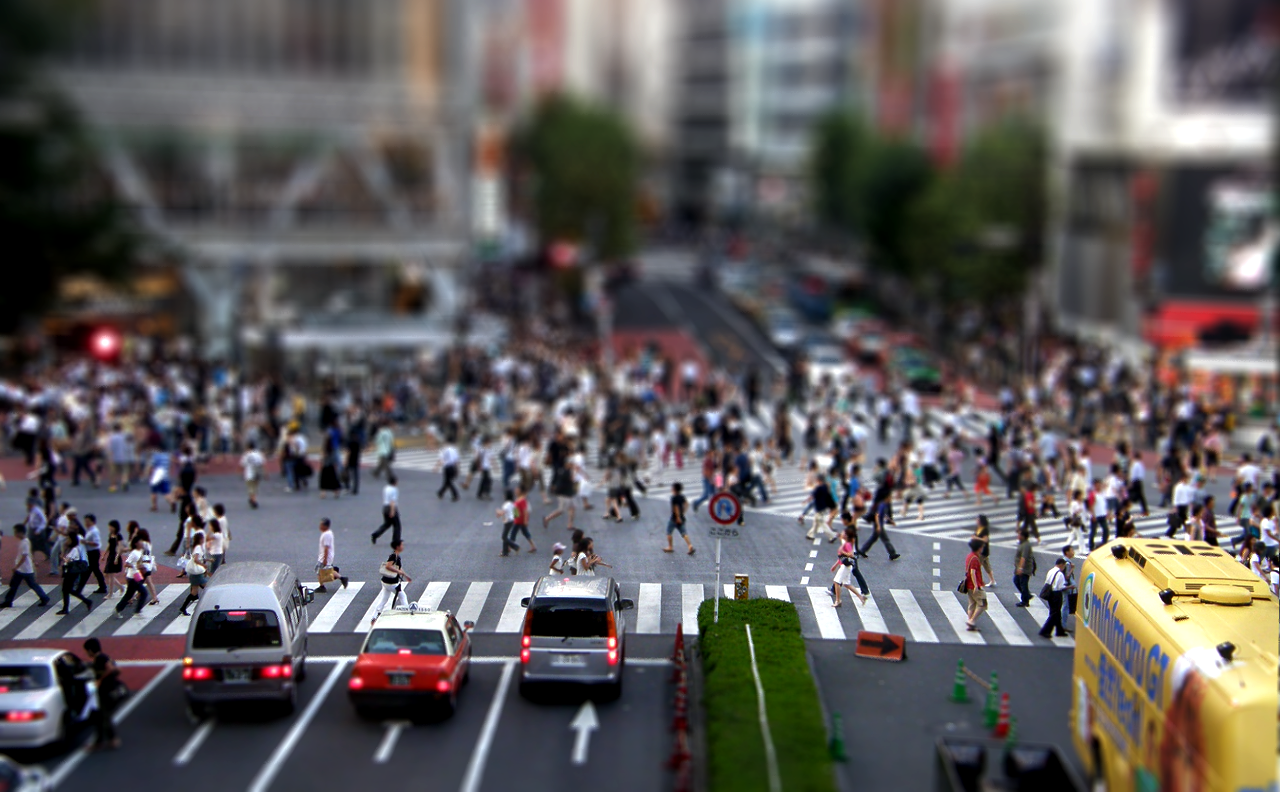
\includegraphics[width=3.35in]{Tilt-Shift-1}
\caption{Durch Postprocessing erzeugter Tilt-Shift-Effekt. Hierbei wurde ein linearer, vertikaler Grauverlauf sowie der von Photoshop CS5 bereitgestellte Linsenfilter mit einem hexagonalen Filterkern verwendet. \\ \small{Die für die Nachbearbeitung verwendete Aufnahme der Shibuya Kreuzung in Tokio wurde vom Flickr-Benutzer Maynard erstellt.}}
\label{flickr}
\end{figure}

Statt auf Tilt-Shift-Objektive zurückzugreifen, kann der beschriebene Effekt gleichwertig mithilfe von linearen Weichzeichnungsfiltern reproduziert werden~\cite{McCloskey:2009ij}. Für die Umsetzung eignet sich ein linearer, vertikaler Grauverlauf zur Beschreibung der Unschärfeintensität für den jeweiligen Bildpunkt. Abbildung \ref{flickr} zeigt eine Aufnahme der Shibuya Kreuzung in Tokio nach Anwendung des Tilt-Shift-Effektes. Dieser wurde auf die beschriebene Art und Weise, nach der Aufnahme des Bildes mit einer handelsüblichen Kamera, durch Postprocessing in Adobe Photoshop CS5 hinzugefügt. Durch die Leichtigkeit und die Wirkung des Effektes, erfreut sich die Erzeugung von Miniaturbildern reger Beliebtheit \cite{Flickr:2011hc}.

Der Einfluss von Unschärfe innerhalb einer Szene auf wahrgenommene Größen- und Abstandsverhältnisse ist unverkennbar. Dennoch kann die Distanz von Objekten zu dem Punkt der Aufnahme einer Fotografie oder Grafik nicht allein anhand der Intensität der Unschärfe rekonstruiert werden. Held. et. al. haben hierzu ein Modell vorgestellt, dass für die Rekonstruktion des Abstandes zur Fokusebene zusätzlich zur Unschärfe relative Distanzen innerhalb der Szene berücksichtigt. Dieses Modell wurde anhand eines semi-automatischen Algorithmus, der Fotografien durch Anwendung von Tiefenschärfe akkurat in gewünschte Größenverhältnisse versetzt, und einem psychophysiologischen Experiment validiert~\cite{Held:2010cr}.

\subsection{Tiefenschärfe in Echtzeit-3D-Applikationen}
Die Berechnung von Tiefenschärfe ist trotz Hardwarebeschleunigung ein rechenaufwändiger Prozess~\cite{Held:2010cr}. Dennoch hat sich der Einsatz von Tiefenschärfe als stilistisches Mittel innerhalb von Computerspielen etabliert und findet zudem bei der Entwicklung von Echtzeit-3D-Applikationen in verschiedenen Formen und Ausführungen Anwendung.

Die erste Variante nutzt die Berechnung des Circle of Confusion (kurz CoC) anhand der Linsengleichung als Grundlage. Dieser gibt für einen betrachteten Punkt unter Berücksichtigung der Brennweite, der Distanz zur Schärfeebene, der relativen Distanz zur Schärfeebene für den betrachteten Punkt und der Größe der Linse, den Durchmesser der Unschärfe an. Nach der Ermittlung des CoC-Wertes wird ein Unschärfefilter mit dem entsprechenden Durchmesser auf jeden Bildpunkt angewandt \cite{Dudash:2004ul,Scheuermann:2004wd}. In Computerspielen wird dieser Effekt meist als stilistisches Mittel verwendet, sodass statt der Linsengleichung lineare Grauverläufe zwischen bestimmten Distanzen interpoliert werden \cite{Earll-Hammon:2007qf,Filion:2008ve}. Zur Verbesserung des Effekts existieren verschiedene Ansätze, um durch das Verfahren bedingte Artefakte zu minimieren.

Unter Verwendung des Circle of Confusion kommt in der Praxis zudem eine rechenaufwändigere Technik zum Einsatz. Bei diesem wird die sogenannte Wärmeleitungsgleichung (engl. heat equation), eine partielle Differentialgleichung, zur Approximation von Unschärfe in einem Punkt verwendet~\cite{Bertalmio:2004lq,Kass:2006dq}. Ausgehend von einem Lochkameramodell wird eine Wärmeverteilung entsprechend den CoC-Werten berechnet \cite{Kass:2006dq}. Für einen großen CoC-Durchmesser wird die thermische Leitfähigkeit des Materials als hoch modelliert und für einen entsprechend kleinen CoC-Durchmesser gering. Dieses Verfahren wird beispielsweise von den Pixar Animation Studios für die Generierung von Echtzeit-Previews genutzt.

Die Publikationen von Sungkil Lee et. al. präsentieren weitere Verfahren zur Echtzeitberechnung von Tiefenschärfe und Unschärfe. Bei einem dieser Verfahren wird der Effekt durch den Einsatz von anisotrophischer Filterung und MIP-Maps erzeugt, wobei mögliche Artefakte durch den Einsatz eines Gauß-Filters unterdrückt werden \cite{Lee:2008nx}. In einem weiteren Verfahren wird die Szene innerhalb eines einzigen Renderingdurchlaufes in mehrere Schichten aufgeteilt. Die Berechnung wird abschließend ähnlich zu Multi-View-Synthesis-Verfahren durchgeführt \cite{Lee:2009eu}. Die aktuelleste Publikation beschreibt ein Renderingsystem, das speziell für die Generierung von Defokussierungs- sowie Unschärfeeffekten entwickelt wurde und zudem die Simulation von verschiedenen Linsenmodellen ermöglicht \cite{Lee:2010oq}.

\subsection{Modell zur Berechnung von Tiefenschärfe}

Die Berechnung des Circle of Confusion bildet die Grundlage für den in diesem Paper vorgestellten Tiefenschärfe-Algorithmus. Die Berechnung dessen baut auf den Ergebnissen von Held et. al. auf~\cite{Held:2010cr}. Eine ideale Linse fokussiert parallel einfallende Lichtstrahlen in einem Punkt $f$, dem sogenannten Brennpunkt. Lichtstahlen, ausgesendet von einem beliebigen Punkt in der Entfernung $z_1$, werden in einem Punkt  $s_1$ auf der entgegengesetzten Seite der Linse fokussiert. Der Zusammenhang zwischen diesen Abständen ist durch die Linsengleichung definiert (Formel \ref{eq:lens}).

\begin{equation}
 \frac{1}{s_1} + \frac{1}{z_1} = \frac{1}{f}
	\label{eq:lens}
\end{equation}

Bei gewöhnlichen Bildaufnahmegeräten liegt die Bildebene parallel zur Linse, sodass Punkte in einer Distanz von $z_0 = ({f^{-1} - {s_0}^{-1}})^{-1}$ im Fokus liegen und somit vollständig scharf dargestellt werden. Die Ebene in der Distanz $z_0$ zur Linse wird als Schärfeebene bezeichnet. Punkte, die nicht auf der Schärfeebene liegen, werden entsprechend unscharf dargestellt. Die Intensität der Unschärfe kann durch den Durchmesser $c$ des Unschärfekreises auf der Bildebene beschrieben werden. Das Verhältnis $\frac{z_1}{z_0}$ (Formel \ref{eq:d}), sprich das Verhältnis von einem Punkt auf der Schärfeebene und einem Punkt, der nicht auf dieser liegt, wird als relative Distanz $d$ bezeichnet. Bei Berücksichtigung des Durchmessers $A$ der Linse ergibt sich für ein Objekt in der Distanz $z_1$ die in Formel \ref{eq:coc} dargestellte Gleichung.

\begin{align}
	 \label{eq:d}
	d &= \frac{z_1}{z_0} \\
	c_1 &= \left| A \frac{s_0}{z_0} ( 1 - \frac{1}{d}) \right|
	\label{eq:coc}
\end{align}

Als Tiefenschärfe (engl. depth of field) wird der Bereich im Umkreis zur Schärfeebene bezeichnet, in dem der Durchmesser $c_1$ so gering ist, dass der betrachtete Punkt vollständig scharf dargestellt wird. Zur Veranschaulichung sind sämtliche, soeben beschriebenen Verhältnisse innerhalb von Abbildung \ref{fig:coc} verbildlicht.

\begin{figure}[htbp]
\centering
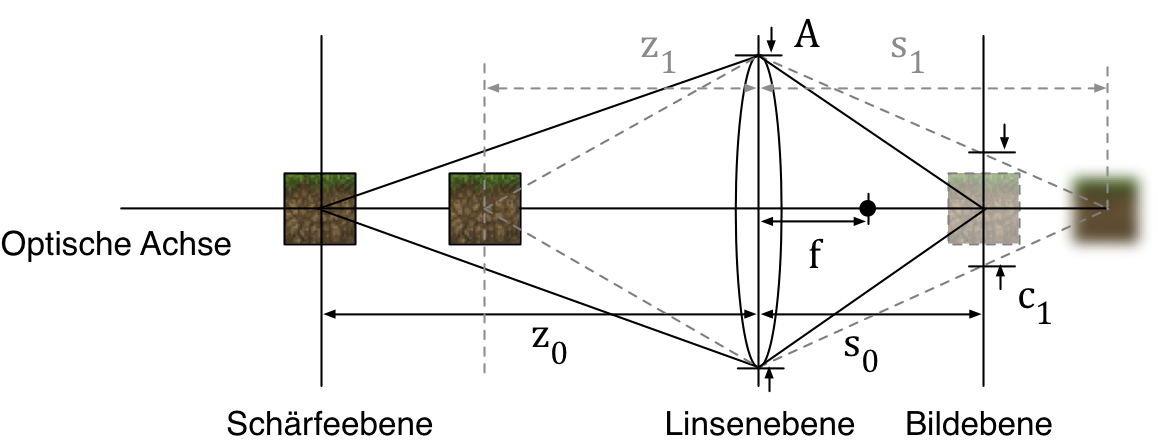
\includegraphics[width=3.35in]{CoC-1}
\caption{Der Circle of Confusion bildet die Grundlage für die Berechnung von Tiefenschärfe. $z_0$ kennzeichnet den Abstand zur Schärfeebene, $A$ die Größe der Linse, $f$ die Brennweite der Linse und $s_0$ den Abstand zwischen Linse und Bildebene. Bei Betrachtung eines Punktes mit der Distanz $z_1$ entsteht ein Streupunkt mit dem Durchmesser $c_1$.}
\label{fig:coc}
\end{figure}

Der zuvor beschriebene Tilt-Shift- bzw. Miniaturisierungseffekt lässt sich mit dem Verhältnis zwischen $z_0$ und $c_1$ erklären. Durch Verringerung von $z_0$, sprich einer Reduzierung des Abstandes zwischen Linse und Schärfeebene, erhöht sich der Durchmesser des Circle of Confusion $c_1$ bei Betrachtung eines Bildpunktes in der relativen Distanz $d$. Entsprechend erzeugt eine aus der Nähe aufgenommene Szene mehr Unschärfe als eine hochskalierte Version der Szene, aufgenommen aus größerer Distanz.

\section{Konzept}

Der vorgestellte Algorithmus basiert, mit kleinen Variatonen, auf dem von T. Scheuermann beschriebenen \emph{Advanced-Depth-of-Field}-Effekt~\cite{Scheuermann:2004wd}. Hierbei werden die eigentlichen Berechnungen in die Grafikpipeline verlagert und in Form von Shadern realisiert. Da der Kernpunkt des Algorithmus die Berechnung des Tilt-Shift-Effektes ist, muss beim Entwurf der Szene darauf geachtet werden, dass die Größenverhältnisse von Entitäten (zumindest näherungsweise) auf die reale Welt übertragbar sind. Um spätere Berechnungen zu erleichtern, sollte eine Einheit der 3D-Umgebung so gewählt werden, dass sie einem Meter in der realen Welt entspricht.

\begin{figure}[htbp]
\centering
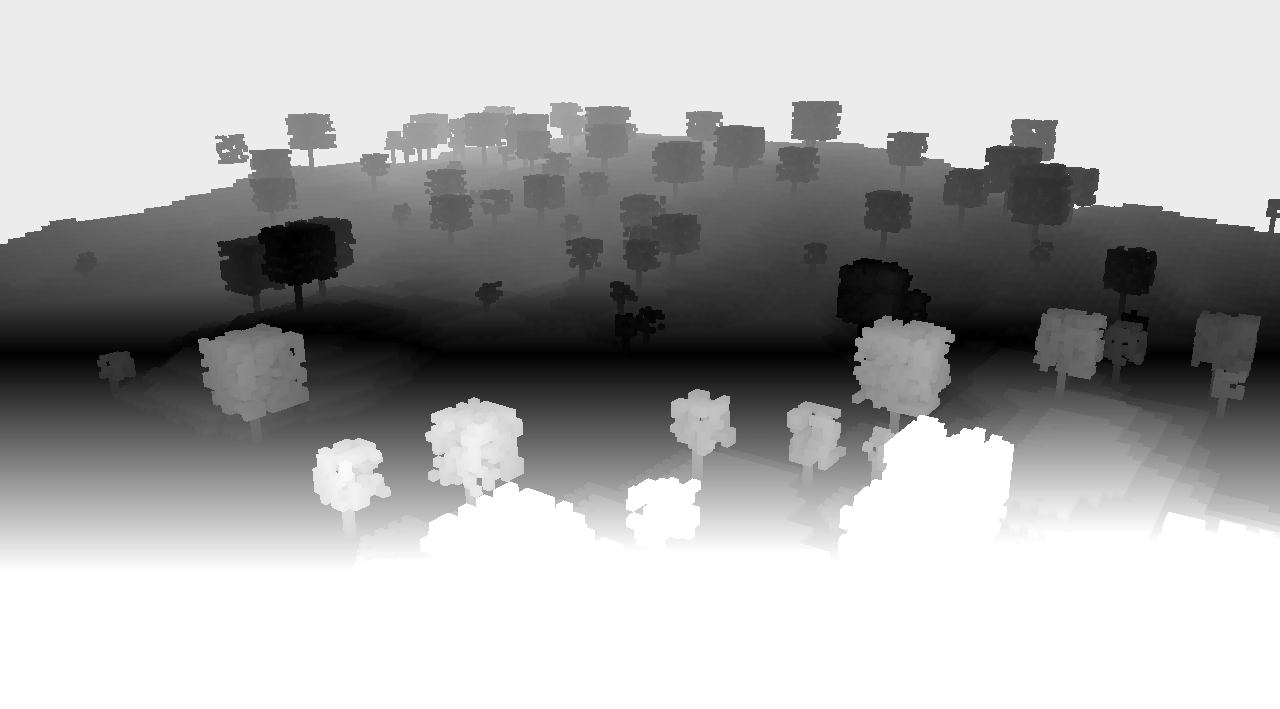
\includegraphics[width=3.35in]{Blockcraft-1-CoC}
\caption{Visualisierung des Circle of Confusion als Grauwertbild. Die Intensität der Unschärfe pro Bildpunkt $c_{x,y}$ wurde skaliert, so dass $c_{x,y} \in [0.0,1.0]$ gilt.}
\label{fig:cocmap}
\end{figure}

Für die eigentliche Berechnung des Echtzeit-Tiefenschärfe-Effektes sind folgende Schritte notwendig: Zunächst müssen die jeweiligen Tiefenwerte für das aktuelle Blickfeld der Kamera ermittelt und für spätere Berechnungen bereitgestellt werden. Im zweiten Schritt muss, ausgehend von den ermittelten Tiefenwerten, der entsprechen Diameter für den Unschärfefilter unter Verwendung der zuvor genannten Formel für $c_1$ (Formel \ref{eq:coc}) für jeden Bildpunkt ermittelt werden. Sowohl die Tiefenwerte als auch die Durchmesserwerte des CoCs werden in der Praxis normalisiert und als Lookup-Table, in Form einer Textur, codiert. Abbildung \ref{fig:cocmap} zeigt die Visualisierung einer solchen Tabelle für den Circle of Confusion als Grauwertbild. 

Anhand der ermittelten Werte für den Circle of Confusion wird im letzten Schritt der eigentliche Tiefenschärfe-Effekt berechnet. Hierzu muss für jeden Bildpunkt entsprechend dem zuvor ermittelten Diameter $c_{x,y}$ ein Unschärfefilter angewendet werden. Die Schwierigkeit liegt an dieser Stelle darin, dass der Durchmesser und die Intensität des Filters variabel wählbar sein muss.

\subsection{Nutzung einer Poisson-Disk-Verteilung als Weichzeichnungsfilter}

Um den Vorgang möglichst effizient zu gestalten, ist von der Verwendung eines Gauß-Filters abzusehen. Für jeden Diameter $c_{x,y}$ müsste an dieser Stelle eine entsprechend große Filter-Matrix bereitgestellt oder dynamisch berechnet werden. Eine Mehrfachausführung des Gauß-Filters ist ebenfalls keine realistische Lösung.

Als geeignete Alternative erweist sich die Poisson-Disk-Verteilung~\cite{Engel:2004uq}. Zur Erzeugung dieser wird zunächst eine Menge von Zufallswerten entsprechend der Poisson-Verteilung generiert. In einem zweiten Schritt werden Punkte eliminiert, die einen bestimmten Mindestabstand zu Nachbarpunkten unterschreiten. Die Poisson-Verteilung eignet sich, bei entsprechender Wahl der Parameter, als Näherung der Gauß-Verteilung, was die Nutzung als Unschärfefilter rechtfertigt. Für die Anwendung als Filterkern werden lediglich Punkte in einem bestimmten Radius betrachtet. Um den Filterkern zu verallgemeinern, ist der Radius des Einheitskreises zu wählen. Die Anzahl der ermittelten Samples ist für die Qualität des Effektes zuständig. Sollten für ein entsprechend großen Radius zu wenige Samples vorhanden sein, können sich im Endergebnis Artefakte in Form von Geisterbildern äußern.

Ausgehend von der Betrachtung eines bestimmten Punktes $\vec{p} = \left(x,y\right)^T$ kann der pro Sample $s_{i}$ zu berücksichtigende Punkt $\vec{p'}$ entsprechend Formel \ref{eq:poissp} ermittelt werden.

\begin{align}
	 \label{eq:poissp}
	\vec{p'} = \vec{p} \cdot s_i \cdot c_{x,y}
\end{align}

Die Farbwerte der entsprechenden Punkte können an dieser Stelle ermittelt und auf den ursprünglichen Punkt aufaddiert werden. Im Anschluss muss der Farbwert lediglich der Anzahl der verwendeten Samples entsprechend normalisiert werden. Abbildungen \ref{fig:poisson} (a) und (b) zeigen die Anwendung eines Filters mit dem Radius $r = 0.0$ bzw. $r = 1.0$ und 6 Samples.

\begin{figure}[htbp]
\centering
\subfigure[]{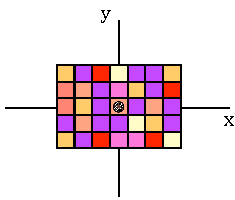
\includegraphics[height=1.25in]{Poisson-1}}
\qquad
\subfigure[]{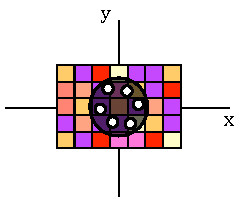
\includegraphics[height=1.25in]{Poisson-2}}
\caption{Anwendung eines Poisson-Disk-Filters mit 6 Samples für einen Radius $r = 0.0$ (a) bzw. $r = 1.0$ (b). Der aktuell betrachtete Bildpunkt liegt im Ursprung des Koordinatensystems.}
\label{fig:poisson}
\end{figure}

\subsection{Simulation des Tilt-Shift-Effektes}
\label{sec:tilt}

Um möglichst wirklichkeitsgetreue Ergebnisse zu erzielen, müssen die Eigenschaften des menschlichen Auges berücksichtigt werden, sodass sich bei Betrachtung von Formel \ref{eq:coc} für $A = \SI{4.6}{\milli\meter}$ und $s_0 = \SI{17.0}{\milli\meter}$ ergeben \cite{Held:2010cr}. 

Für die Simulation des Tilt-Shift-Effektes muss nun die Größe der Linse, ausgehend von den ursprünglichen Dimensionen, angepasst werden. Bei Simulation einer Distanz, die um Faktor $m$ verschoben wird, ergibt sich das in Formel \ref{eq:zhat} und \ref{eq:ahat} beschriebene Verhältnis~\cite{Held:2010cr}.

\begin{align}
	 \label{eq:zhat}
	\hat z_0 &= m \cdot  z_0 \\
	 \label{eq:ahat}
	\hat A &= \frac{A}{m}
\end{align}

Geht man beispielsweise von $s_0 = \SI{0.017}{\meter}$ sowie $A = \SI{0.0046}{\meter}$ und einer Szene, die aus einer Distanz $z_0 = \SI{75.0}{\meter}$ aufgenommen wurde, aus, muss für die Simulation einer Distanz von $\hat z_0 = \SI{0.06}{\meter}$ eine Linse mit $\hat A = \SI{5.75}{\meter}$ verwendet werden.

\subsection{Abbildung der Größenverhältnisse}
\label{sec:proportions}

Unter Berücksichtigung der zuvor beschriebenen Parameter für die menschliche Wahrnehmung und Formel \ref{eq:coc}, kann der Durchmessers des Circle of Confusion bei einer Projektion auf die menschliche Netzhaut berechnet werden. Für eine Simulation muss die Verbindung zwischen dem beschriebenen Durchmesser des Poisson-Disk-Filters und dem Durchmesser des CoCs hergestellt werden. Hierzu wurden die Ergebnisbilder von Held et. al. betrachtet und der jeweilige Durchmesser des angewendeten Filters anhand eines Gauß-Weichzeichnungs-Filters approximiert \cite{Held:2010cr}. Mithilfe von Photoshop CS5 wurde für eine der beschriebenen Szenen aus einer simulierten Distanz $\hat z_0 = \SI{0.06}{\meter}$ mit $\hat A = \SI{60.0}{\meter}$, $z_0 = \SI{785.0}{\meter}$, $s_0 = \SI{0.017}{\meter}$ und $A = \SI{0.046}{\meter}$ ein maximaler Unschärfe-Radius von $r = \SI{4.6}{px}$ ermittelt. Bei Anwendung des Poisson-Disk-Filters muss für den Durchmesser des maximalen CoCs $c_{\textnormal{max}} = \SI{4.6}{px} \cdot 2 = \SI{9.2}{px}$ gewählt werden.

\begin{figure}[htbp]
\centering
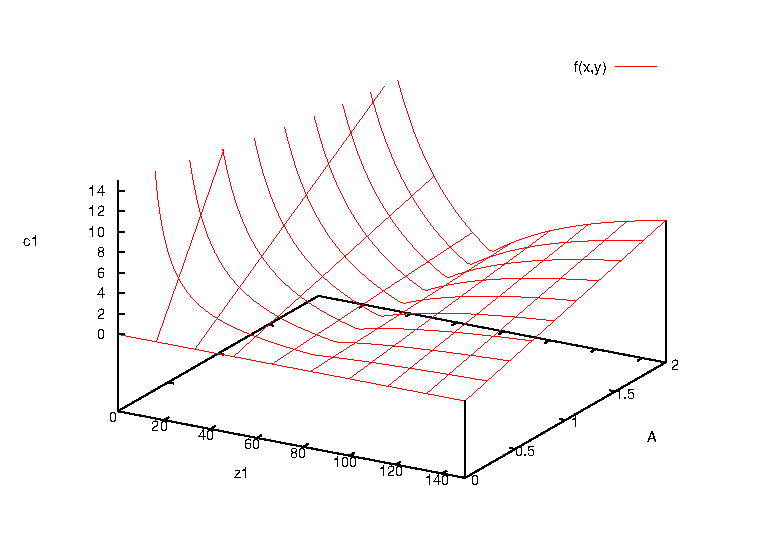
\includegraphics[width=3.35in]{DoF-Graph}
\caption{Durchmesser des CoCs für eine Linse der Größe $A \in [\SI{0.0}{\meter},\SI{2.0}{\meter}]$, $z1 \in [\SI{0.0}{\meter},\SI{150}{\meter}]$, $z_0 = \SI{75.0}{\meter}$, $s_0 =\SI{0.017}{\meter}$ bei Verwendung des Skalierungsfaktors $b = 28000$.}
\label{abb:cocgraph}
\end{figure}

Anhand der Parameter der betrachteten Beispielszene kann der Skalierungsfaktor $b = 28000$ geschätzt werden. Unter Verwendung dessen entspricht die Intensität der dargestellten Unschärfe in etwa der, die bei Betrachtung der Szene aus der simulierten Distanz tatsächlich entstehen würde~\cite{Held:2010cr}. Abbildung \ref{abb:cocgraph} zeigt den Durchmesser des CoC für ein Beispielszenario nach Anwendung der beschriebenen Skalierung.

\section{Berechnung der Tiefenschärfe mithilfe von Shadern}

Für die Implementierung des Tiefenschärfe-Effektes kommen zwei spezifische Fragment-Shader und ein Vertex-Shader zum Einsatz. Der Vertex-Shader ist für die Erzeugung der Tiefenwerte zuständig, während die zwei Fragment-Shader für die Berechnung der CoC-Werte und die Anwendung des eigentlichen Tiefenschärfe-Effektes zuständig sind. Anhand der ermittelten Werte wird eine Depth-Map bzw. CoC-Map erzeugt, wobei die CoC-Map an den finalen Shader für die Berechnung des Tiefenschärfe-Effektes übergeben wird. In diesem kommen die erzeugten Maps zusammen mit einer Textur, die ein Rendering der betrachteten Szene beinhaltet, zur Erzeugung des finalen Tiefenschärfe-Effektes zur Verwendung.

Bei der Realisierung des Effektes wird davon ausgegangen, dass die Werte des Z-Puffers nicht unmittelbar zur Verfügung stehen und diese zunächst mithilfe eines entsprechenden Shaders ermittelt werden müssen. 

\subsection{Erzeugung der Depth-Map}
\label{sec:depthmap}

Der Vertex-Shader für die Depth-Map muss auf sämtliche Vertices der Szene angewendet werden. Ausgehend von einem Punkt in Weltkoordinaten, wird eine Transformation in das Kamerakoordinatensystem und abschließend in das Projektionskoordinatensystem durchgeführt. Hierzu müssen die entsprechenden Matrix-Transformationen der Reihe nach oder in Form einer einzigen Matrix, oft als World-View-Projection-Matrix oder Model-View-Projection-Matrix bezeichnet, ausgeführt werden.

Nach der Ermittlung der Koordinaten des Vertex muss, um die Darstellung als Graubild zu ermöglichen, der entsprechende Wert auf der Z-Achse des Koordinatensystems auf einen Bereich zwischen $0.0$ und $1.0$ abgebildet werden. Ein Tiefenwert von $1.0$ steht hierbei für sehr nahe und $0.0$ für  Punkte in der maximal möglichen Entfernung. Dies kann durch eine Beschränkung der Auflösung erreicht werden, bei der die maximal darstellbare Tiefe der Szene entsprechend festgelegt wird. Der Dividend muss für spätere Berechnungen und die Rückrechnung in die Ausgangseinheit bereitgestellt werden. 

Listing \ref{lst:depth} zeigt eine mögliche Implementierung eines entsprechenden Shaders in Pseudocode. 

\begin{lstlisting}[caption=Pseudocode fur den Vertex-Shader zur Erzeugung der Depth-Map.,language=pseudo,label={lst:depth}]
vertex program DepthVertexShader with parameters worldPosition, worldViewProjectionMatrix, sceneDepth
	set position to worldViewProjectionMatrix * worldPosition 
	set colour to 1.0 - position.z / sceneDepth
	
	return saturate (colour) and position
end
\end{lstlisting}

Der ermittelte Farbwert muss mithilfe eines Fragment-Shaders ausgegeben werden. Da dieser sehr einfach umzusetzen ist, wird an dieser Stelle auf eine detaillierte Beschreibung verzichtet.

\subsection{Erzeugung der CoC-Map}

Unter Verwendung der zuvor beschriebenen Depth-Map (siehe Abschnitt \ref{sec:depthmap}) wird nun innerhalb eines Fragment-Shaders die Gleichung für $c_1$ (siehe Formel \ref{eq:coc}) zur Berechnung der CoC-Map eingesetzt. Hierzu wird für jeden Pixel der Ausgabetextur der entsprechende Wert für $c_1$ als Grauwert kodiert. Da die Unschärfeintensitäten bei Verwendung der Parameter des menschlichen Auges je nach Abstand verschwindend gering ausfallen, muss der Wert vor der eigentlichen Ausgabe skaliert werden (mit Hinblick auf die Genauigkeit von einfachen Gleitkommazahlen). Diese Skalierung muss bei einer erneuten Verwendung berücksichtigt werden.

Listing \ref{lst:coc} zeigt eine exemplarische Implementierung eines entsprechenden Fragment-Shaders als Pseudocode.

\begin{lstlisting}[caption=Pseudocode für den Fragment-Shader zur Berechnung der CoC-Map.,language=pseudo, label={lst:coc}]
fragment program DepthFragmentShader with parameters currentPoint, depthSample, z0, a, sceneDepth
	// z0 entspricht z.B. 32.0
	// a entspricht z.B. 0.0046
	set s0 to 0.017
	set depthValue to depthSample at currentPoint
	set d to ( sceneDepth * ( 1.0 - depthValue) ) ) / z0
	set cocDiameter to absolute ( a * ( s0 / z0 ) * ( 1.0 - ( 1.0 / d ) ) ) * 1000.0;
	
	return saturate ( cocDiameter );
end
\end{lstlisting}

\subsection{Abschließende Berechnung des Tiefenschärfe-Effektes}

Abschließend wird nun unter Verwendung der CoC-Map, einem Abbild der aktuell betrachteten Szene als Textur und unter Verwendung einer im Voraus definierten Menge von Poisson-Disk-Samples der Tiefenschärfe-Effekt für jeden Bildpunkt berechnet. Hierzu wird vom aktuell betrachteten Bildpunkt für jedes Sample der zu betrachtende Punkt gemäß Formel \ref{eq:poissp} berechnet, die entsprechenden Farbwerte addiert, normalisiert und der finale Farbwert zurückgegeben. Unter Berücksichtigung von Abschnitt \ref{sec:proportions} muss an dieser Stelle der Skalierungsfaktor $b = 28000$ bei Berechnung des CoC-Diameters berücksichtigt werden.

An dieser Stelle wird davon ausgegangen, dass die Poisson-Samples an die Darstellungsauflösung der Szene angepasst sind und der Multiplikator in Pixeln beschrieben werden kann.

Listing \ref{lst:dof} zeigt eine exemplarische Implementierung eines entsprechenden Fragment-Shaders als Pseudocode.

\begin{lstlisting}[caption=Pseudocode für den Fragment-Shader zur Berechnung der Tiefenschärfe.,language=pseudo,label={lst:dof}]
fragment program DepthOfFieldFragmentShader with parameters currentPoint, depthSample, cocSample, sceneSample
	set cocValue to cocSample at currentPoint
	set cocDiameter to (cocValue / 1000.0) * 28000
	set result to 0.0 0.0 0.0

	for each point p in poissonSamples do
		set newPoint to currentPoint + p * cocDiameter
		set result to result + sceneSample at newPoint
	end
	
	return normalize ( result )
end
\end{lstlisting}

\section{Ergebnisse}

Die Referenzimplementierung wurde mithilfe von Ogre (Kurzform für \emph{Object-Oriented Graphics Rendering Engine})~\cite{Torus:2011vn} unter Verwendung von Mac OS 10.6.6 und OpenGL sowie der Shader-Hochsprache Cg (Kurzform für \emph{C for Graphics}) durchgeführt. Als Grafikkarte wurde eine ATI Radeon 5870 mit 1 GB Grafikspeicher eingesetzt. Der Testrechner besitzt einen Intel Xeon 6-Kern-Prozessor mit 3.33 GHz pro Kern, 12 Threads und insgesamt 8 GB Arbeitsspeicher. Für die Darstellung wurde ein Weitbildmonitor mit ein Bilddiagonalen von $24''$ und einer Auflösung von $1920\times\SI{1200}{px}$ verwendet.

Die beschriebenen Shader wurden mithilfe des von Ogre bereitgestellten Material- sowie Kompositor-Systems zugeordnet. Da die Tiefenwerte getrennt von der eigentlichen Berechnung ermittelt werden müssen, wird eine sogenannte Render-Queue-Invocation verwendet, bei der der Shader für die Erzeugung der Depth-Map auf die Szenen-Objekte angewendet und das Gesamtergebnis in Form einer Textur für die weitere Verwendung vorbereitet wird. Für den Unschärfefilter wurden 32 Poisson-Disk-Samples pro Frame verwendet, wobei der Tiefenschärfe-Shader zur Verstärkung des Effektes zweifach ausgeführt wird.

Für die Demonstration wurde eine spezielle Szene entwickelt, die einen \emph{Lego-Effekt} vermitteln soll. Die Szene besteht aus vielen einzelnen, quadratischen Blöcken, die durch einen fraktalen Algorithmus (dem Square-Diamond-Algorithmus) zu einem Terrain ausgelegt werden. Zudem werden für bestimmte, zufällig ermittelte Regionen, Seen und Schneeabschnitte erzeugt sowie Bäume in der Landschaft platziert. Die Szene besteht aus Blätter-, Sand-, Dreck-, Schnee-, Gras-, Holz- sowie Wasserblöcken, die mit einfachen Texturen à $16\times\SI{16}{px}$ versehen wurden. Die Dimensionen eines Blockes wurden so gewählt, dass die Proportionen geschätzt einem halben Meter in der realen Welt entsprechen. Bäume besitzen eine maximale Höhe von  $\approx \SI{6.00}{\meter}$. Der Stil der Beispielszene orientiert sich am Computerspiel Minecraft~\cite{Mojang:2011zr}. Zur Verdeutlichung des Effektes kann sich innerhalb der Szene frei bewegt und bei Bedarf auf eine Vogelperspektive umgeschaltet werden. Abbildung \ref{abb:block} zeigt eine Aufnahme der Szene aus der Betrachtersicht.

\begin{figure*}[p]
	\centering
	\subfigure[See mit $z_0 = \SI{75.0}{\meter}$ und $A = \SI{4.6}{\milli\meter}$]{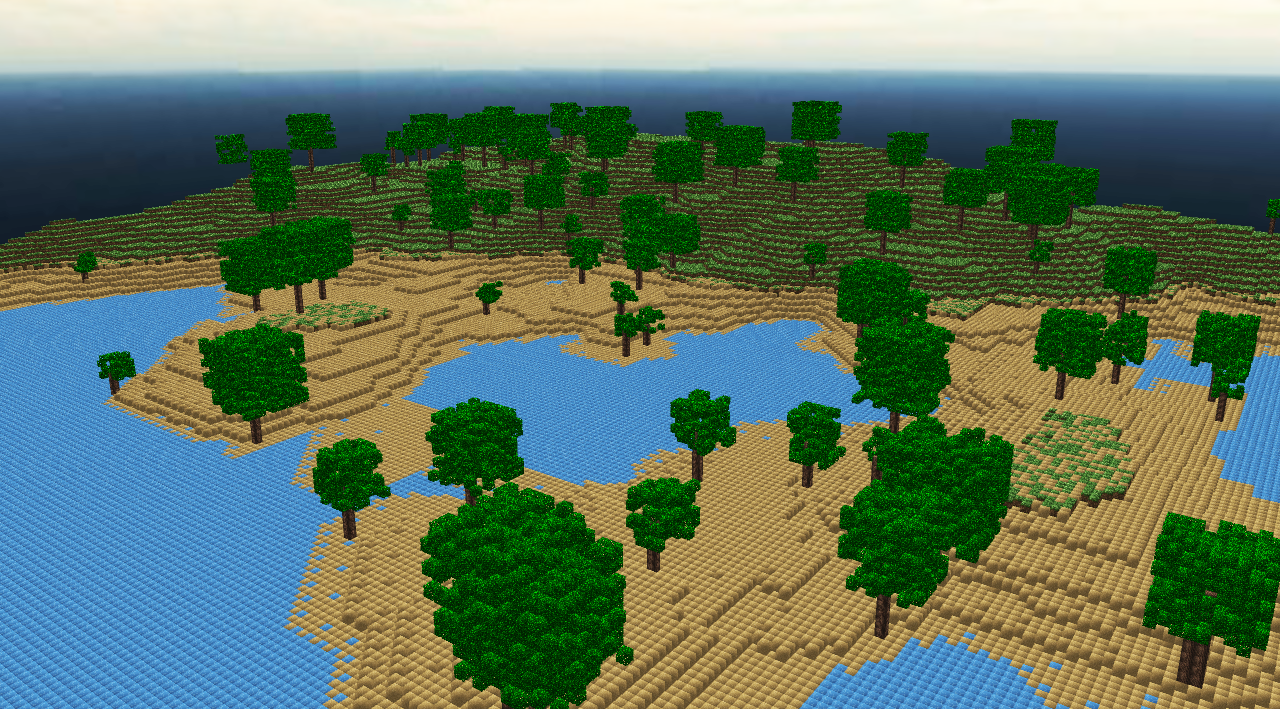
\includegraphics[height=1.75in]{Blockcraft-1-Original}}
	\qquad
	\subfigure[Wald mit $z_0 = \SI{75.0}{\meter}$ und $A = \SI{4.6}{\milli\meter}$]{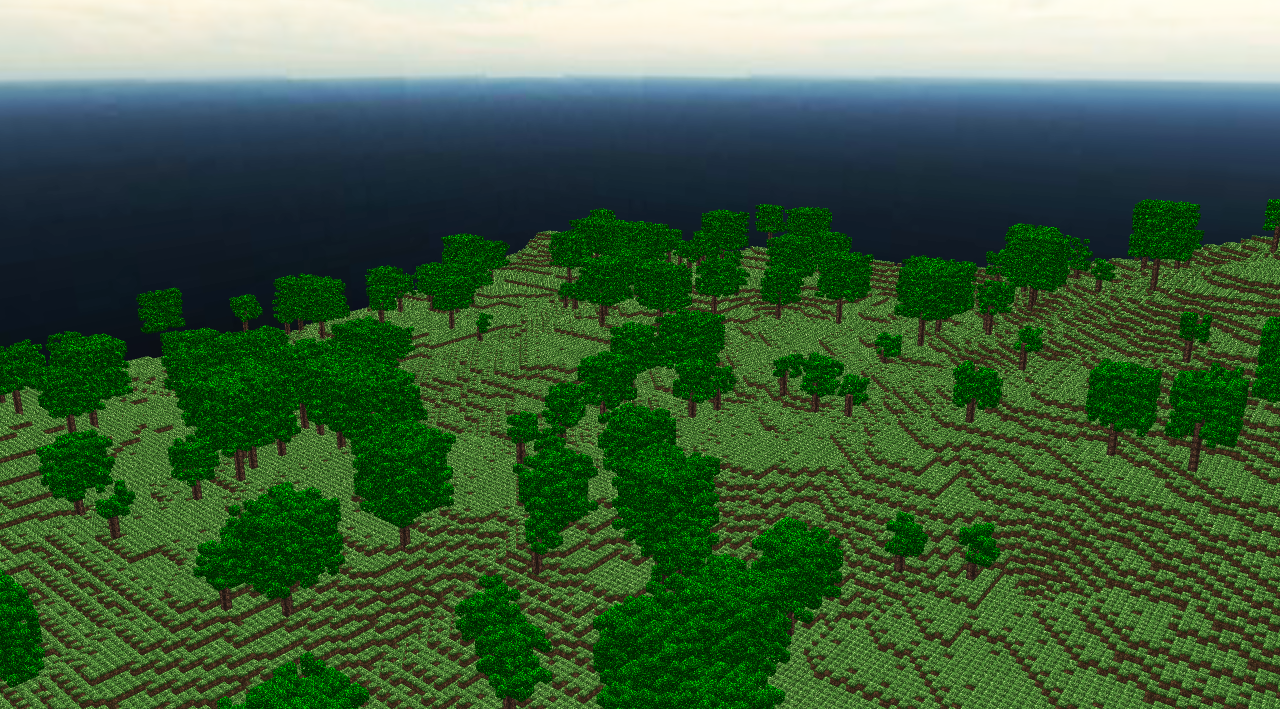
\includegraphics[height=1.75in]{Blockcraft-2-Original}}
	\qquad
	\subfigure[See mit $\hat z_0 = \SI{6.0}{\centi\meter}$ und $\hat A = \SI{5.75}{\meter}$]{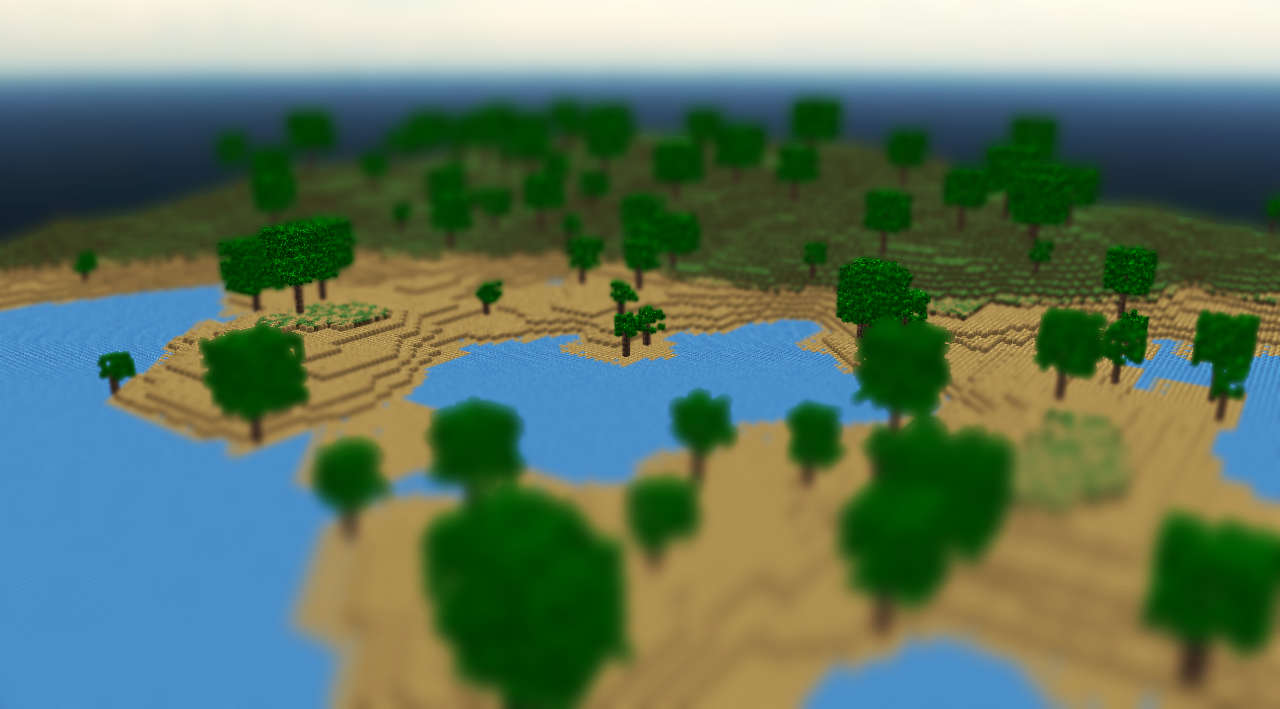
\includegraphics[height=1.75in]{Blockcraft-1-Blur}}
	\qquad
	\subfigure[Wald mit $\hat z_0 = \SI{6.0}{\centi\meter}$ und $\hat A = \SI{5.75}{\meter}$]{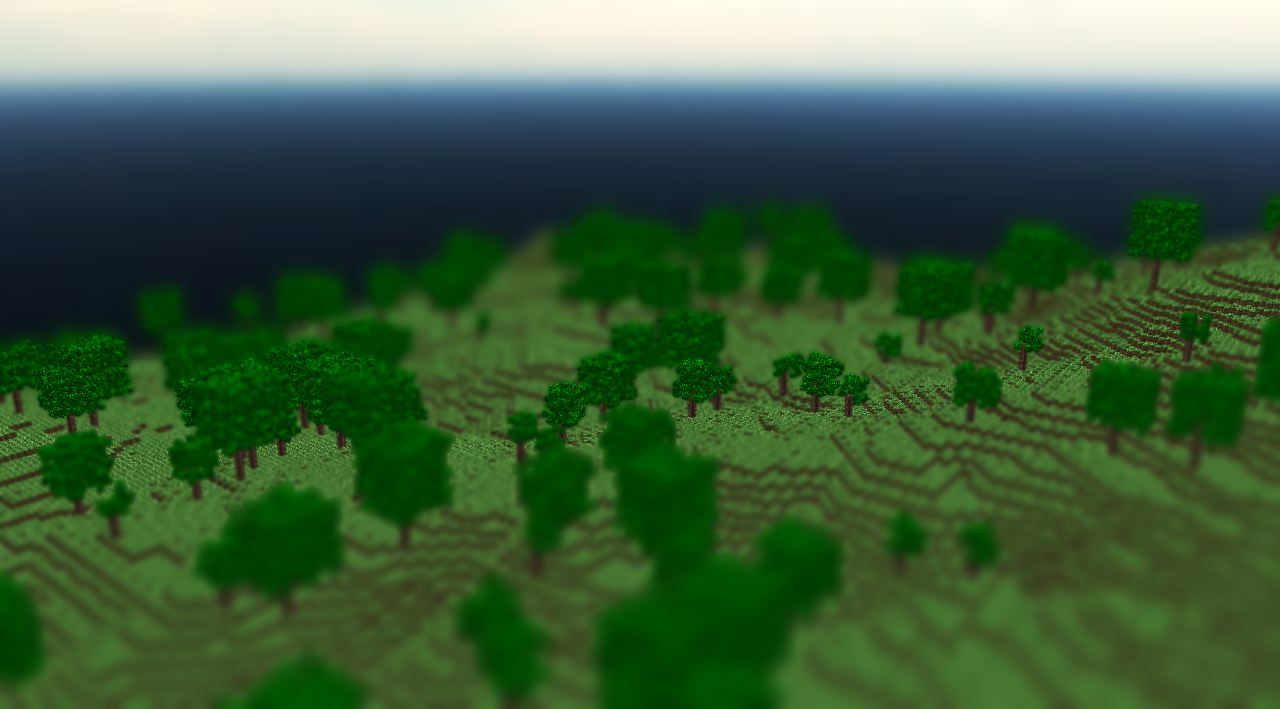
\includegraphics[height=1.75in]{Blockcraft-2-Blur}}
	\qquad
	\subfigure[See mit linearem, vertikalem Linsenfilter]{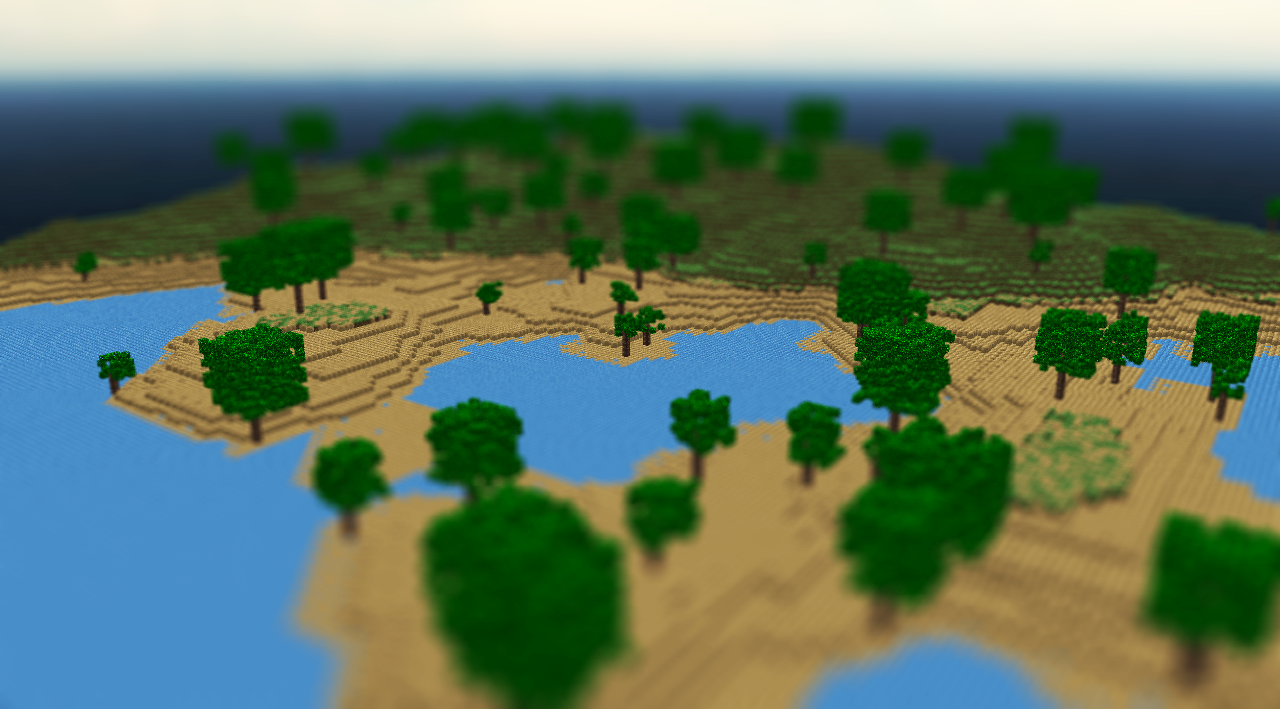
\includegraphics[height=1.75in]{Blockcraft-1-Photoshop}}
	\qquad
	\subfigure[Wald mit linearem, vertikalem Linsenfiler]{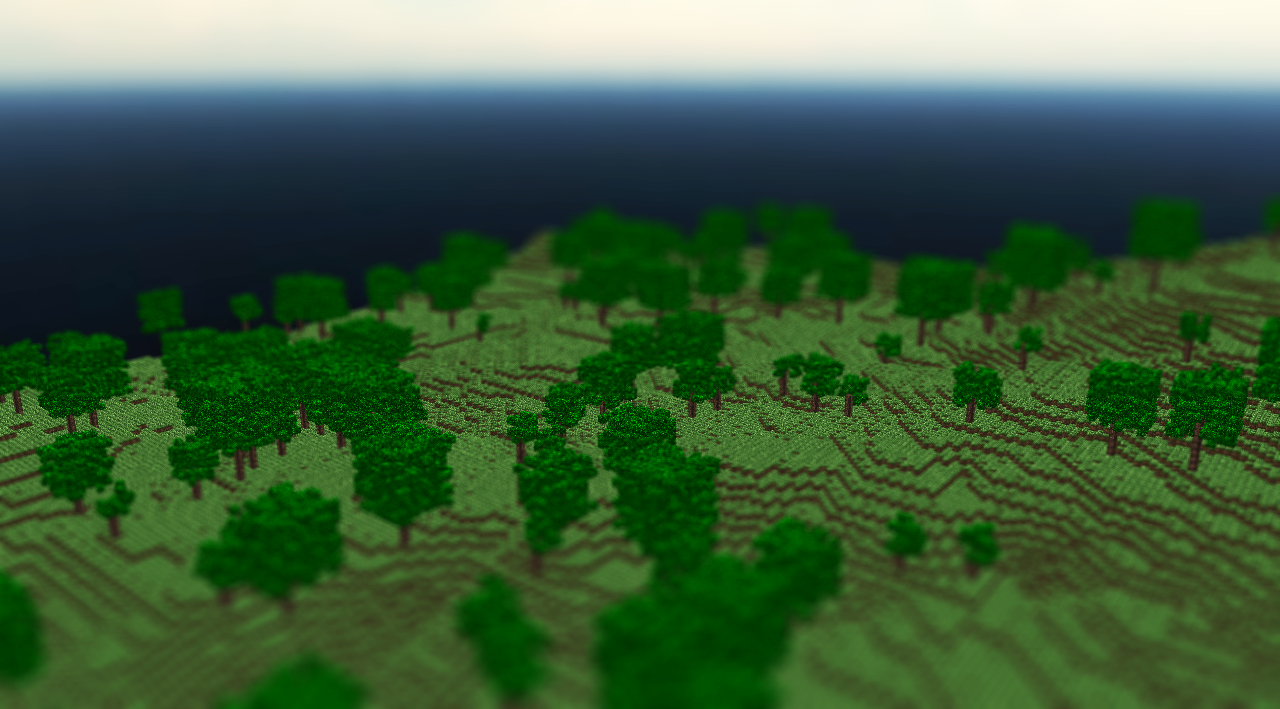
\includegraphics[height=1.75in]{Blockcraft-2-Photoshop}}
\caption{Zu Demonstration des Algorithmus wurden zunächst zwei Bilder aus einer großen Distanz von $\SI{75.0}{\meter}$ aufgenommen (a und b). Im Anschluss daran wurde mithilfe des vorgestellten Algorithmus eine Simulation einer Distanz von ca. $\SI{6.0}{\centi\meter}$ durch Vergrößerung der Linse durchgeführt (c und d). Zum Vergleich wurde ausgehend von der CoC-Karte der Ergebnisse ein linearer Grauverlauf abgeschätzt und zur Weichzeichnung mithilfe des Linsenfilters von Adobe Photoshop CS5 verwendet (e und f).}
	\label{abb:res}
\end{figure*}

Abbildungen \ref{abb:res} (a) und (b) zeigen die Anwendung des Tiefenschärfe-Effektes aus einer Distanz von ca. \SI{50.0}{\meter} zur Oberfläche in zwei unterschiedlichen Regionen. Abbildung \ref{abb:res} (c) und (d) zeigen die gleichen Szenen bei Betrachtung aus einer simulierten Distanz von \SI{6.0}{\centi\meter} zur Schärfeebene. Abbildungen \ref{abb:res} (e) und (f) zeigen zum Vergleich die Anwendung eines linearen Unschärfefilters, der nach dem in Abbildung \ref{flickr} gezeigten Verfahren mithilfe eines linearen, vertikal verlaufenden Weichzeichnungsfilters erzeugt wurde.

\begin{figure}[htbp]
\centering
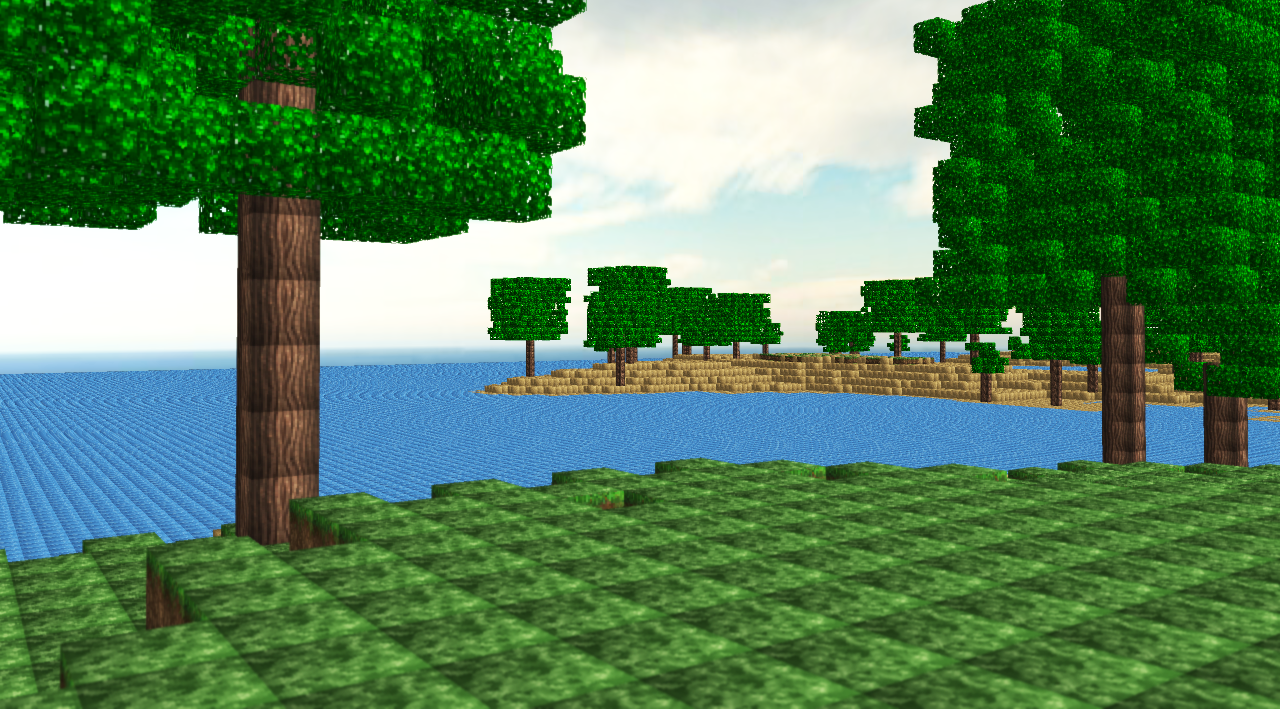
\includegraphics[width=3.35in]{Blockcraft-1}
\caption{Blick in die Beispielszene bei normalen Größenverhätltnissen.}
\label{abb:block}
\end{figure}

Die Beispielanwendung wird ohne Anwendung des Tiefenschärfe-Effektes bei einer Darstellung eines Gebietes von $512 \times 512$ Blöcken mit $52$ Frames pro Sekunde (kurz FPS) ausgeführt. Nach Anwendung des Effektes sinkt der Wert auf $51\;\textnormal{FPS}$.

\section{Diskussion}

\begin{figure*}[p]
	\centering
	\subfigure[]{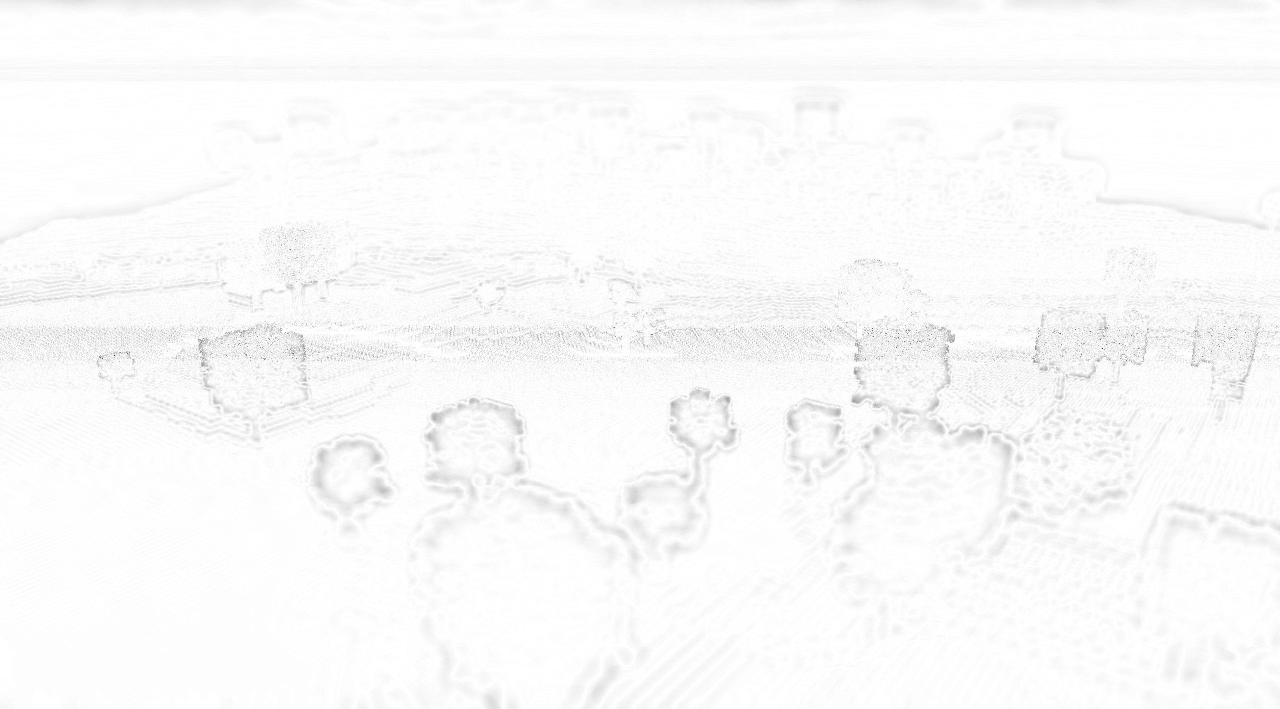
\includegraphics[height=1.75in]{Blockcraft-1-Difference}}
	\qquad
	\subfigure[]{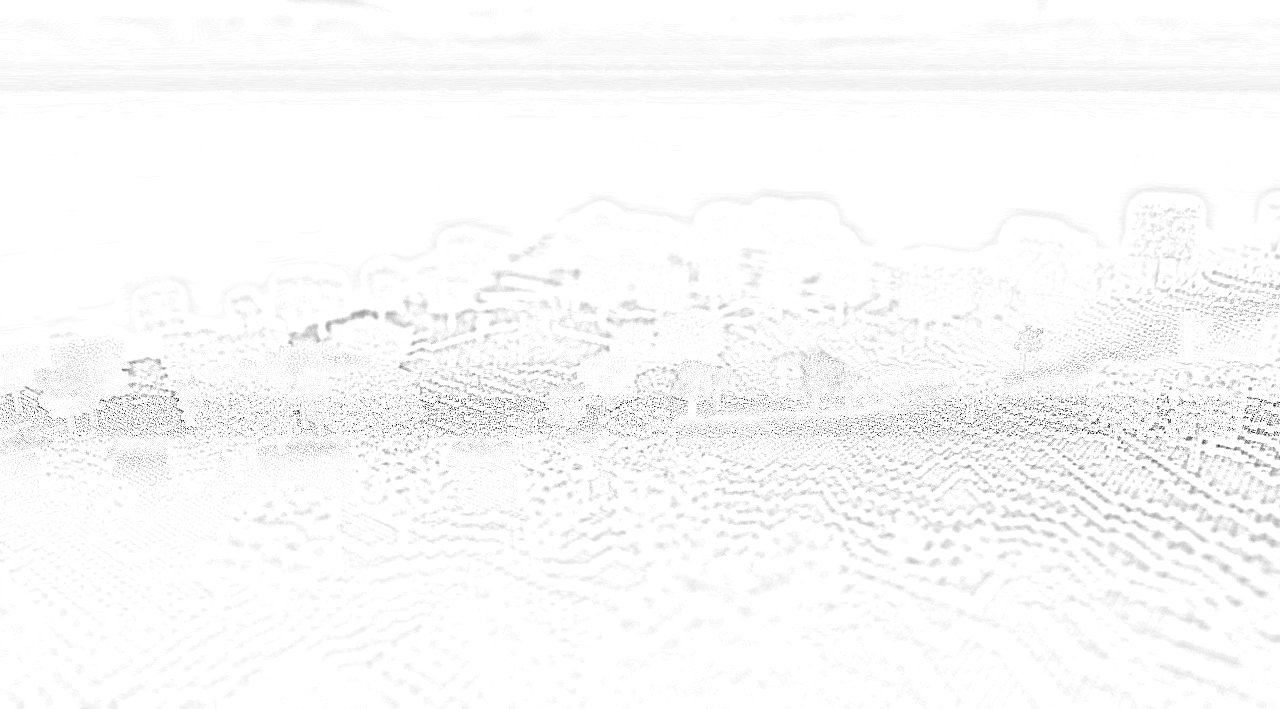
\includegraphics[height=1.75in]{Blockcraft-2-Difference}}
\caption{Farbdifferenzbilder der Beispielszenen zur Verdeutlichung der Unterschiede zwischen dem vorgestellten Echtzeit-Tiefenschärfe-Effekt und der Offline-Berechnung mittels Photoshop.}
	\label{abb:diff}
\end{figure*}

Die Ergebnisse, nach Anwendung des beschriebenen Echtzeit-Tiefenschärfe-Effektes, entsprechen den Erwartungen. Die durch die Anwendung des Tilt-Shift-Effektes entstehenden Größenverhältnisse sind, aus subjektiver Sicht, korrekt und lassen sich mit einem Vergleich zu den von Held et. al. bereitgestellten Referenzbildern bestätigen. Der entstehende Effekt ist somit nicht nur für photorealistische Szenen interessant, sondern kann auch, wie durch die von uns vorgestellte Beispielszene bewiesen wird, auf synthetische Szenarien übertragen werden.

Im Vergleich zu einem nachträglich auf das Bild angewendeten Linsenfilter (siehe Abbildung \ref{abb:res}), ergeben sich nur wenig Differenzen. Da das vorgestellte Verfahren physikalisch korrekt unter der Verwendung von Tiefenwerten arbeitet, kann ein genaueres Ergebnis erzielt werden. Dies äußert sich darin, dass, bei Nutzung des linear verlaufenden Unschärfeffektes, Objekte, die eigentlich auf der Schärfeebene liegen müssten, unscharf dargestellt werden und vice versa. Betrachtet man beispielsweise in Abbildung \ref{abb:res} (e) einen der Bäume im Bereich der Fokusebene, kann es zur Weichzeichnung von Baumspitzen kommen, obwohl diese bei Betrachtung der Tiefenwerte auf der Schärfeebene liegen müssten.

Die beschriebenen Effekte können den in Abbildung \ref{abb:diff} gezeigten Farbdifferenzbildern entnommen werden. Deutliche Unterschiede sind innerhalb der Bilder schwarz hervorgehoben, während schwache oder nicht vorhandene Unterschiede als grau bzw. weiß zu erkennen sind. Das vorgestellte Verfahren zeigt, zusammen mit vielen weiteren Verfahren, Artkefakte an den Übergängen zwischen Vordergrundebene, Schärfeebene und Hintergrundebene. Objekte, die im Vordergrund im äußeren Bereich der Schärfeebene liegen und die Schärfeebene überlagern, erhalten eine harte Kante, da der Unschärfefilter lediglich einzelne Punkte innerhalb der CoC-Map betrachtet. Zudem lässt sich ein \emph{Ineinanderbluten} beobachten, da für die Erzeugung des Unschärfeeffektes die Farbwerte der umliegenden Pixel benötigt werden. Dieser Effekt tritt ebenfalls am Übergang zwischen Schärfe- und Hintergrundebene auf, was zu einer Art \emph{Glühen} an scharf dargestellten Entitäten führen kann.

\section{Zusammenfassung und Ausblick}

Innerhalb des vorliegenden Papers wurde ein Verfahren vorgestellt, das die Berechnung eines Tiefenschärfe-Effektes unter Berücksichtigung der Eigenschaften des menschlichen Auges in Echtzeit ermöglicht. Unter Verwendung dessen kann der sogenannte Tilt-Shift-Effekt physikalisch korrekt reproduziert und auf synthetische Szenen angewendet werden.

Das vorgestellte Verfahren basiert auf der Verwendung von Tiefenwerten zur Ermittlung des Circle of Confusion anhand der Linsengleichung. Um eine korrekte Abbildung erzeugen zu können, werden die Eigenschaften des menschlichen Auges berücksichtigt. Die Simulation verschiedener Effekte wird durch die Anpassung der Linsengröße durchgeführt.

Ausgehend von den Ergebnissen dieses Papers, kann das vorgestellte Verfahren auf erweiterte Algorithmen, wie zum Beispiel den Einsatz der Wärmeleitungsgleichung~\cite{Bertalmio:2004lq,Kass:2006dq} zur Minimierung von Artefakten durch das Einbeziehen von benachbarten Punkten bei der Anwendung der Unschärfe, übertragen werden. Hierbei muss jedoch beachtet werden, dass erweiterte Verfahren deutlich höhere Anforderungen an die Leistung des Grafikprozessors stellen und für komplexe Szenarien ungeeignet sind.

% \begin{figure}[p]
% \centering
% 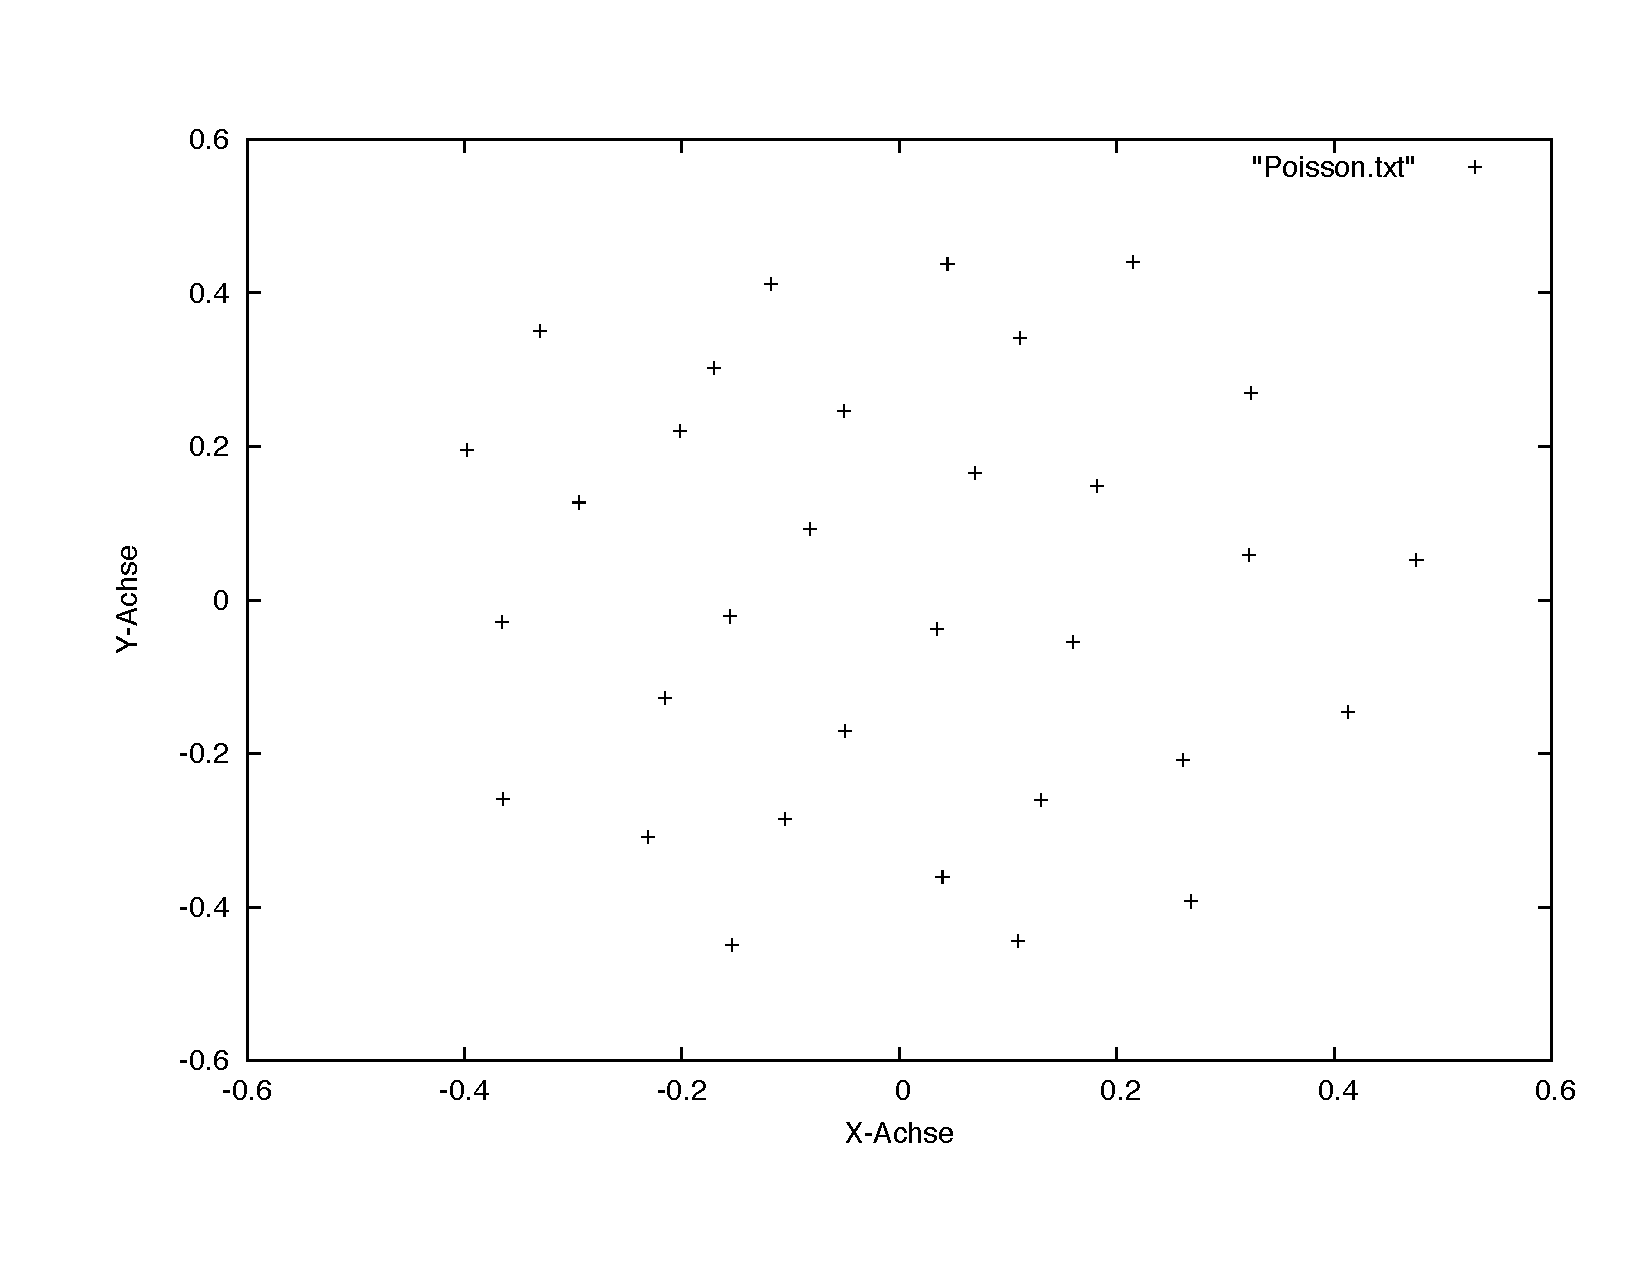
\includegraphics[width=3.35in]{Poisson-Distr}
% \caption{Die verwendete Poisson-Disk-Verteilung mit 32 Samples.}
% \label{abb:poissond}
% \end{figure}

\bibliographystyle{acmsiggraph}
\nocite{*}
\bibliography{Literatur}
\end{document}
